\chapter{Inference in BN}
\label{cha:inter_BN}

The criteria with which a Bayesian Network (Chapter \ref{cha:bay_net}) is built,
allows us to get information about the data.\\

We assume that we have evidence $e$ (what I observe) on the state of a subset of
variables $E$ in the model. Therefore Inference amounts as computing the posterior
probability of a subset $X$ of the non-observed variables given the observation:
\[
	P(X|E = e)
\]
Inference is computing the probability of variable $X$ (one of more non-observed
variables) given the observed variables (posterior probability of $X$ given the evidences).\\

A graphical model is designed as a network of joint probability, we can use
messages to compute joint probability of the variable of interest and the
evidence. Typically I need the conditional probability, then I need to compute (Bayes'
theorem \ref{theo:bayes}):
\[
	P(X | E = e) = \frac{P(X, E=e)}{P(E=e)}
\]
Then I need to compute $P(X, E=e)$ and $P(E=e)$, the denominator is easy (once I
compute the numerator $P(E=e) = \sum_{X}P(X, E=e)$ (through a marginalization)),
therefore I need to compute the nominator.\\ The nominator is a joint
probability, I want to exploit the BN structure to compute this numerator easily,
otherwise it will explode exponentially. For this reason, we can exploit the
structure of the Bayesian Network to get inference more easily, this will end up
in a problem that can be solved using dynamic programming.

\section{Inference in chain-like structure}
Let's start from a linear chain of nodes, which will be our BN (Bayesian Network).
\begin{figure}[H]
	\centering
	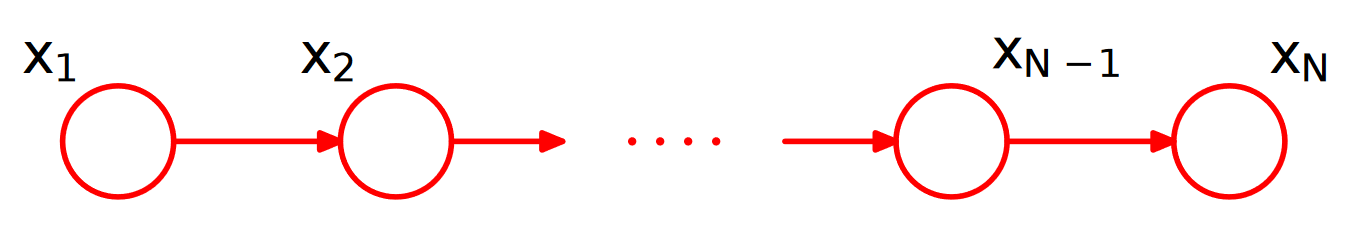
\includegraphics[scale=0.3]{
		images/09_BayesianNetworksInference_chainInference.png
	}
\end{figure}
We want to compute the probability for a certain node given some evidence:
\[
	P(X| E=e) = \frac{P(X, E=e)}{P(E=e)}
\]

\subsection{Inference without evidence}
Let's ignore the evidence first, then come back to that later. The probability of
any of the nodes depends on the previous nodes as The joint distribution modelled
on the BN is $P(X_{1}, \dots, X_{n})$, then if I am interested in $P(X_{n})$ I
know that it possibly depends on all the other possible variables (marginalization)
This is where the exponential problem would come up.
\[
	P(X_{n}) = \sum_{X_i \neq X_n}P(X_{1}, \dots, X_{n})
\]
Considering joint probability decomposed according to the chain is
\[
	P(X_{n}) = \sum_{X_1}\sum_{X_2}\dots \sum_{X_{n-1}}\sum_{X_{n+1}}\sum_{X_n}P(X_{1}
	)P(X_{2}|X_{1})P(X_{3}|X_{2})\dots P(X_{n}|X_{n-1})
\]
But we notice that the sum over $X_{n}$ has only a value in the decomposition which
depends on it ($P(X_{n}|X_{n-1})$), the other probabilities are constant with
respect to $X_{n}$. Therefore we represent this value as a function depending on
$X_{n-1}$
\[
	\mu_{\beta} (X_{n-1}) = \sum_{X_n}P(X_{n}|X_{n-1})
\]
So we get
\[
	P(X_{N}) = \sum_{X_1}\sum_{X_2}\dots \sum_{X_{n-1}}P(X_{1})P(X_{2}|X_{1})P(X_{3}
	|X_{2})\dots P(X_{n-1}|X_{n-2}) \mu_{\beta} (X_{n-1})
\]
We can proceed with the same intuition for all the previous members
\[
	\mu_{\beta} (X_{i}) = \sum_{i+1}P(X_{i+1}|X_{i})\mu_{\beta}(X_{i+1})
\]
I go back with this procedure until $n+1$.\\

We can compute a similar procedure from the top to the bottom of the chain. Given
\[
	P(X_{n}) = \sum_{X_1}\sum_{X_2}\dots \sum_{X_{n-1}}P(X_{1})P(X_{2}|X_{1})P(X_{3}
	|X_{2})\dots P(X_{n}|X_{n-1})
\]
notice that the terms that depend on the first summation $\sum_{X_1}$ are only $P
(X_{1})P(X_{2}|X_{1})$, then we can carry on the same reasoning
\[
	\mu_{\alpha} (X_{2}) = \sum_{X_1}P(X_{1})P(X_{2}|X_{1})
\]
where $\alpha$ stands for forward messages while $\beta$ for reverse messages.
\[
	\sum_{X_2}\sum_{X_2}\dots \sum_{X_{n-1}}\mu_{\alpha}(X_{2}) P(X_{3}|X_{2}) \dots
	P(X_{n}|X_{n-1})
\]
In general:
\[
	\mu_{\alpha} (X_{i}) = \sum_{X_{i-1}}\mu_{\alpha}(X_{i-1}) P(X_{i}|X_{i-1})
\]
For the forward message we can stop when
\[
	\mu_{\alpha} (X_{n}) = \sum_{X_{n-1}}\mu_{\alpha} (X_{n-1}) P(X_{n}|X_{n-1})
\]
The only term that is left from the two chain is $P(X_{n})$ that can be written
as
\[
	P(X_{n}) = \mu_{\alpha} (X_{n}) \mu_{\beta}(X_{n})
\]
this means that computing the local probabilities and summing them independently,
using (for a binary problem) a number of operation equal to $2(n-1)$ instead of $2
^{n}$. $\mu_{\alpha}$ and $\mu_{\beta}$ are message sent backwards or forward
from node to node. The message is always a function of the destination node: I
am interested in computing the probability of the $i^{th}$ node and I collect
the messages coming from the adjacent nodes.
\begin{figure}[H]
	\centering
	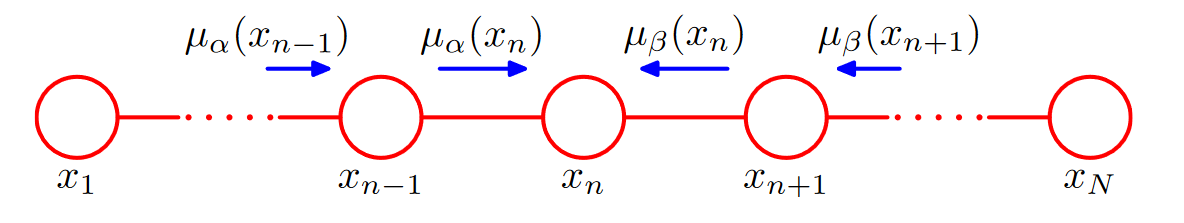
\includegraphics[scale=0.3]{
		images/09_BayesianNetworksInference_messagePassingChain.png
	}
	\caption{Inference for the $i^{th}$ node based on the messages from the
	previous and next node passing}
	\label{fig:message_passing_inference_BN_chain}
\end{figure}
Nodes compute messages to be sent to the next node, as generalization, the message
computed is a combination of a local probability of that node and the message received
from the previous (or next) nodes: this is a standard way to send messages also
for non-chain structures.\\

It is clever to store the partial computations we can do the \textit{full
message passing}: sending a message from the top to the end of the chain and vice
versa, so we have already computed all the partial computation that we could
need.\\

\subsection{Inference adding evidence}
Typically we have some observed values, and then we want to compute the
probability: instead of the sum over the values for the variable that I observed
we can plug in the value I actually observed.\\ Let's say I observed $X_{1} = x_{e1}
, X_{3} = x_{e3}$ in a chain of 4 elements and I what to compute $X_{2}$. This
can be done as
\[
	P(X_{2}|X_{3} = x_{e3}, X_{1} = x_{e1}) = \frac{P(X_{1}, X_{2}, X_{3}, X_{4})}{P(X_{3}
	= x_{e3}, X_{1} = x_{e1})}
\]
the joint probability can be computed as
\[
	\sum_{X_4}P(X_{1}, X_{2}, X_{3}, X_{4}) = P(X_{1} = x_{e1}, X_{2}, X_{3} = x_{e3}
	, X_{4})
\]
where for the observed values I can plug in the values
\[
	\sum_{X_4}P(X_{1} = x_{e1})P(X_{2}|X_{3} = x_{e3}, X_{1} = x_{e1})P(X_{3} = x_{e3}
	))P(X_{4}|X_{3} = x_{e3})
\]
The only term that depends of $X_{4}$ is the last probability, therefore
\[
	\sum_{X_4}P(X_{4}|X_{3} = x_{e3}) = \mu_{\beta}(X_{3} = x_{e3})
\]
and for the latter I do have the value observed. The inference procedure is
actually the same, having evidence implies plugging in values instead of computing
a summation.\\

After all it is true that:
\begin{equation}
	P(X_{n}|\textbf{X}_{e} = \textbf{x}_{e}) = \frac{P(X_{n}, \textbf{X}_{e} =
	\textbf{x}_{e})}{\sum_{X_n}P(X_{n}, \textbf{X}_{e} = \textbf{x}_{e})}
\end{equation}
with bold values as evidence.

\section{Inference in trees-like structure}
The solution highlighted for chains can be extended to trees. At this point we
should consider different kind of structures:
\begin{figure}[H]
	\centering
	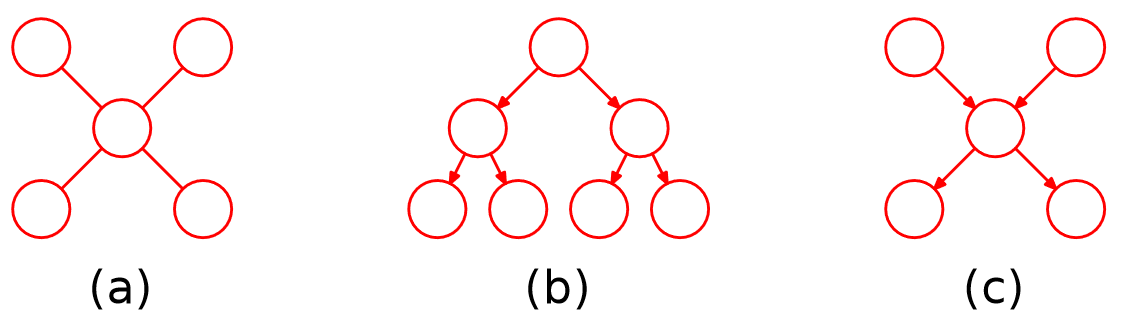
\includegraphics[scale=0.3]{
		images/09_BayesianNetworksInference_treesInferences.png
	}
	\caption{a) undirected trees b) directed trees c) directed poly-trees}
	\label{fig:trees_structure}
\end{figure}

\begin{enumerate}[label=(\alph{*})]
	\item \textbf{undirected trees}: undirected graph with a single path for each pair
		of nodes

	\item \textbf{directed trees}: directed graph with a single node (root) with no
		parents, all other nodes with a single parent

	\item \textbf{directed poly-trees}: directed graphs with multiple parents, for
		node and multiple roots but still a single (undirected) path between each
		pair of nodes.
\end{enumerate}

The procedure that we will described will work for directed (BN) and undirected models
(Markov's Models, \textit{MM}).\\

In order to facilitate the description (and the implementation) we need to go
through an alternative representation of the graphical model: a \textit{factor
graph}. \defi{\textbf{Factor graph}\label{def:factor_graph}\\ It is a graphical representation of a graphical model highlighting its factorization. The factor graph is an undirected graph that has one node for each node in the original graph and also additional nodes for each factor (a factor node had undirected links to each of the node variables in the factor). }
\begin{figure}[H]
	\centering
	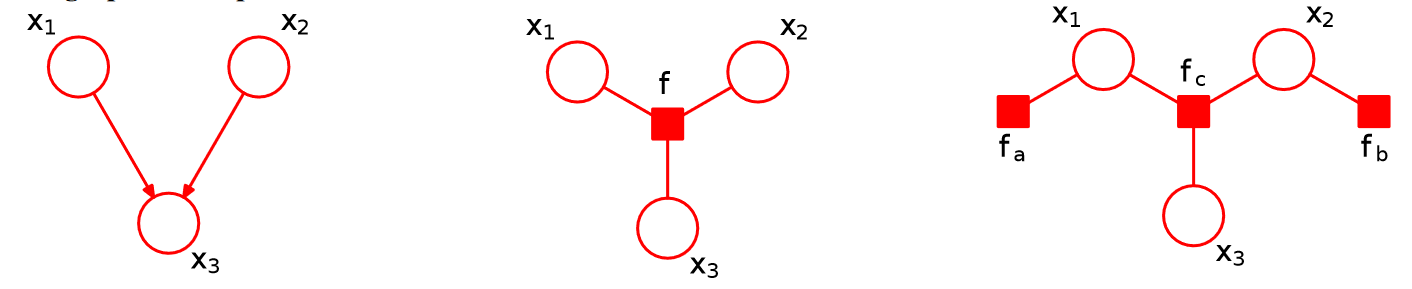
\includegraphics[scale=0.3]{
		images/09_BayesianNetworksInference_factorGraph.png
	}
	\caption{Example of two different factor graphs for the first directed graph.}
	\label{fig:factor_graph}
\end{figure}
A factor is a component of the joint distribution we are trying to represent. The
value associated to the factor is a probability distribution. In Figure
\ref{fig:factor_graph} we can look at two different realization of factor graphs
for the easy directed graph on the left. The factor graph in the middle represent
the following factorialization: \\
$f(x_{1}, x_{2}, x_{3}) = p(x_{3}|x_{1}, x_{2})P(x_{1})P(x_{2})$\\ while the most
right one stands for \\ $f_{a}(x_{1}) = P(x_{1})$\\ $f_{b}(x_{2}) = P(x_{2})$\\ $f
_{c}(x_{1}, x_{2}, x_{3}) = p(x_{3}|x_{1}, x_{2})$\\ This last one means that \\
$P(x_{1}, x_{2}, x_{3}) = f_{c}(x_{1}, x_{2}, x_{3})f_{a}(x_{1})f_{b}(x_{2})$\\ The
latter is the one that we will use ad default option since is the most complete.

\subsection{The sum-product algorithm}
If we think of the inference algorithm on chain, we took the incoming message, multiply
over the local probability, summing over one variable and sending the message to
another variable (\textit{sum-product alternation}): this procedure is efficient
for tree-like structure (also chain as edge case).\\ On factor graphs it still
can be applied if the factor graph it belongs to one of the classes described in
Figure \ref{fig:trees_structure} (a factor graph will not be directed).

\subsubsection{Inference without evidence}
At this point I have no evidence, and no sequence. I have a generic joint
probability (marginalize on everything except $X$ in which I am interested)
\[
	P(X) = \sum_{\textbf{X} \neq X}p(\textbf{X})
\]
Let us remind that in the chain case
\[
	P(X_{n}) = \mu_{\alpha} (X_{n}) \mu_{\beta}(X_{n})
\]
This version is the same but generalized to all the messages reaching the node (incoming),
the node are only connected to factors (not nodes) therefore it is the product for
all factors in the neighbourhood from the factor to $X$
\[
	P(X) = \prod_{f_s \in adj(X)}\mu_{f_s \rightarrow X}
\]
where $f_{s} \rightarrow X$ stand for $f_{s}$ as source and $X$ as destination.
The message is always a function of the variable \textit{node} because the factor
has more variables.
\begin{figure}[H]
	\centering
	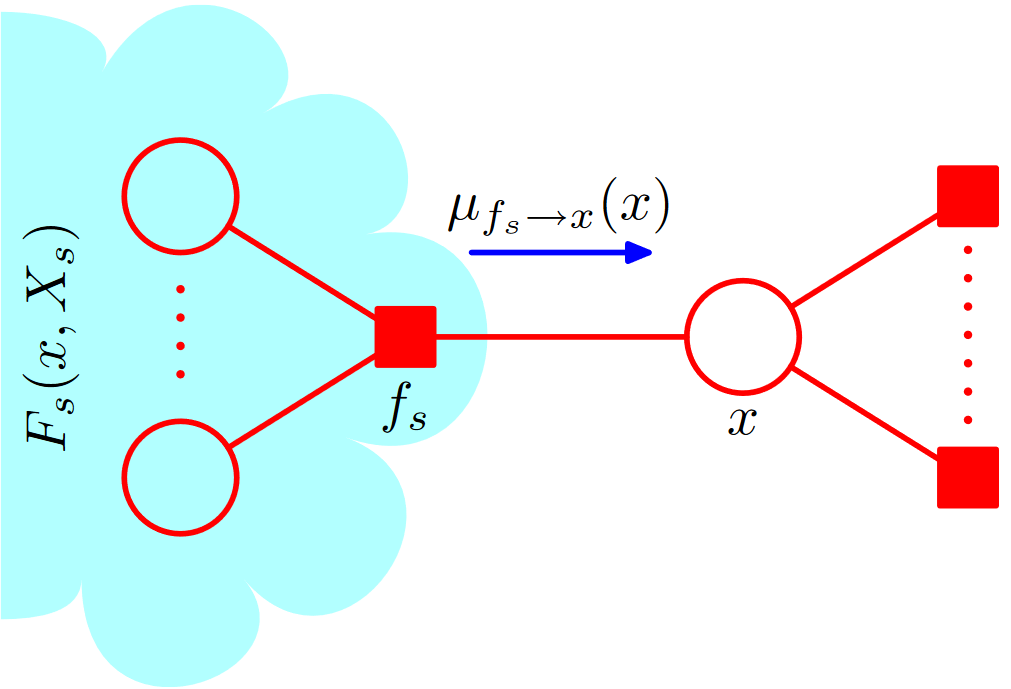
\includegraphics[scale=0.3]{
		images/09_BayesianNetworksInference_forwardMessagePassing.png
	}
	\caption{Collecting messages from the adjacent nodes of X (fwd message passing)}
	\label{fig:message_BN_fwd}
\end{figure}
The value corresponding to the message that $f_{s} \rightarrow X$ is the
multiplication of the incoming messages from its adjacent nodes multiplied by
the local probability of the factor.
\[
	\mu_{f_s \rightarrow X}= \sum_{X_1}\dots\sum_{X_{m}}f(X, X_{1}, \dots, X_{m}) \prod
	_{X_i \in adj(f_s) \neq X}\mu_{X_i \rightarrow f_s}
\]
with $x_{1}, \dots, x_{m}$ the nodes that $f_{s}$ receives messages from (but
the destination $X$).\\

Computing the message from the node to a factor becomes simple: I have a node that
needs to send a message to a factor, then it will be connected only to factors
node $f_{1}, \dots, f_{n}$. The message from $f \rightarrow X$ is always a function
of the variable node, then we
\begin{itemize}
	\item collect messages from the adjacent nodes, therefore multiply for all
		factors that are not the destination (this is the \textbf{product of the
		incoming messages} for all neighbours)
		\[
			\mu_{X \rightarrow f}(X) = \prod_{f_i \in adj(X) \neq X}\mu_{f_i
			\rightarrow X}(X)
		\]

	\item if the messages is at the extremes, then we need to take care of leaves.
		We start sending messages from the leaves $X$, then the message will be
		equal to one since it has no incoming messages
		\[
			\mu_{X \rightarrow f}(X) = 1
		\]

	\item if the extreme is a factor, then we will not have any incoming messages
		and from this
		\[
			\mu_{f \rightarrow X}= \sum_{X_1}\dots\sum_{X_{m}}f(X, X_{1}, \dots, X_{m})
			\prod_{X_i \in adj(f) \neq X}\mu_{X_i \rightarrow f}
		\]
		we get that it is only function of one variables
		\[
			\mu_{f \rightarrow X}= f(X)
		\]
\end{itemize}
We can start sending messages like this, and then things come together as sums and
products.\\

The message computation in a tree structure gets more complicated than a chain (in
which it is enough to start from top and end of the chain). Given a tree, we
have a root already defined, but in the factor graph we do not.\\ Therefore we take
one node (whatever) and use it as a root so we have leaves defined. From the
leaves we send messages and each node will send messages further up. At some point
the messages will reach the root. At this point we can compute the probability
of the root as the product of the messages coming to the root.

\sumup{Therefore the procedure for computing the probability for a generic node, is using it as root, making leaves send messages and eventually getting the messages from the adjacent factors of the node we are interested in.}

In order to avoid useless computation, we send all messages up to the root, then
from the root we send messages all down to the leaves. The same for the intermediate
nodes: this is a \textit{full messages passing scheme}. At this point we do not
care about who the root is because we will have received all partial messages to
all nodes and factors in each direction. Therefore we can compute whatever we want.\\

\subsubsection{Example of inference without evidence}
Let's consider the following graph as an example:
\begin{figure}[H]
	\centering
	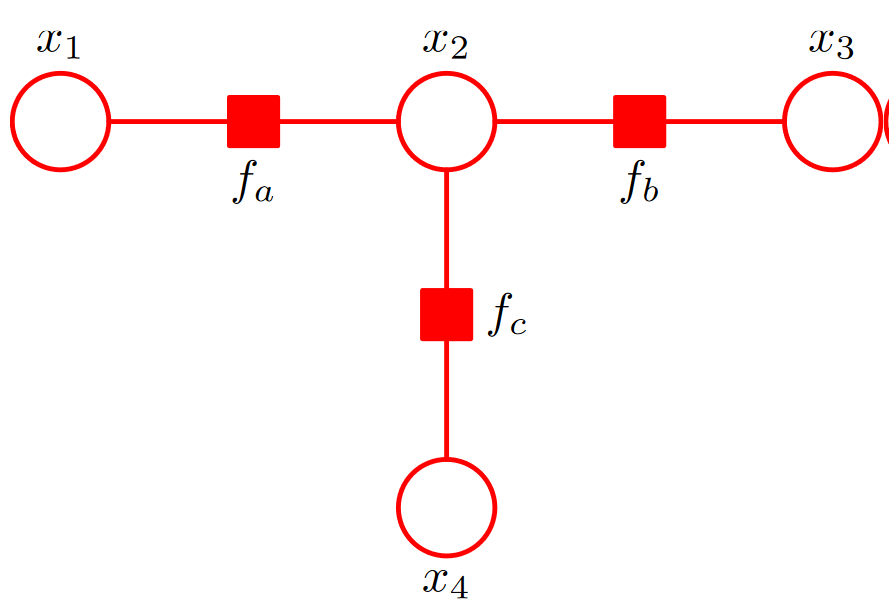
\includegraphics[scale=0.25]{
		images/09_BayesianNetworksInference_exampleInference.png
	}
	\caption{Example graph}
	\label{fig:example_graph_inference_BN}
\end{figure}
The joint probability encoded in this factor graph is the product of the three factors,
with $f_{a}(x_{1}, x_{2}), f_{b}(x_{2}, x_{3}), f_{c}(x_{4}, x_{2})$. Therefore it
is the multiplication
\[
	P(X) = f_{a}(x_{1}, x_{2}) f_{b}(x_{2}, x_{3}) f_{c}(x_{4}, x_{2})
\]
Let's do inference choosing $x_{3}$ as root (by chance), then $x_{1}, x_{4}$ are
leaves. $x_{1}, x_{4}$ can start sending messages to the root $x_{3}$. Since
$x_{1}, x_{4}$ are (leaf) nodes, then their message is equal to 1
\[
	\mu_{x_1 \rightarrow f_a}(x_{1}) = 1
\]
\[
	\mu_{x_4 \rightarrow f_c}(x_{4}) = 1
\]
Once these messages are received by $f_{a}, F_{c}$, then the factors can send
messages to the next nodes.
\begin{align*}
	\mu_{f_a \rightarrow x_2}(x_{2}) & = \mu_{x_1 \rightarrow f_a}(x_{1}) \sum_{x_1}f_{a}(x_{1}, x_{2}) \\
	                                 & = \sum_{x_1}f_{a}(x_{1}, x_{2})
\end{align*}
and
\begin{align*}
	\mu_{f_c \rightarrow x_2}(x_{2}) & = \mu_{x_4 \rightarrow f_c}(x_{4}) \sum_{x_4}f_{c}(x_{4}, x_{2}) \\
	                                 & = \sum_{x_4}f_{c}(x_{4}, x_{2})
\end{align*}
At this point $x_{2}$ received two messages and can compute its own message to send
to $f_{b}$ as
\begin{align*}
	\mu_{x_2 \rightarrow f_b}(x_{2}) & = \mu_{f_a \rightarrow x_2}(x_{2}) \mu_{f_c \rightarrow x_2}(x_{2})
\end{align*}
And now $f_{b}$ sends its message to $x_{3}$ multiplying it by its internal factor
\[
	\mu_{f_b \rightarrow x_3}(x_{3}) = \mu_{x_2 \rightarrow f_b}(x_{2}) \sum_{x_2}f
	_{b} (x_{2}, x_{3})
\]
This is the message reaching $x_{3}$, which has only one neighbour, so its probability
it is only the incoming message $\mu_{f_b \rightarrow x_3}(x_{3})$. Replacing
bits of equations we get
\[
	P(x_{3}) = \sum_{x_1}\sum_{x_2}\sum_{x_4}f_{a}(x_{1}, x_{2}) f_{b}(x_{2}, x_{3}
	) f_{c}(x_{4}, x_{2})
\]
Please notice that the result is as expected the sum over all the variables
except the destination. At this point we can propagate backwards until every node
received messages from all neighbours.

\subsubsection{Another example}
Let's consider now the following graph with its factor graph
\begin{figure}[H]
	\centering
	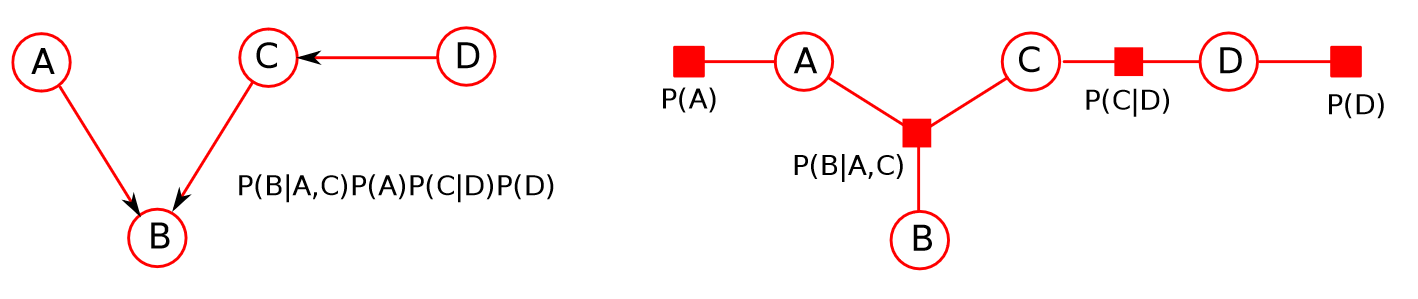
\includegraphics[scale=0.3]{
		images/09_BayesianNetworksInference_exampleInferenceEvidence.png
	}
	\caption{Example graph with possible factor graph}
	\label{fig:inference_graph_evidence}
\end{figure}
Suppose we want to compute the probability for $B$. What we do is sending
messages towards $B$ (both factors and intermediate nodes). Nodes $A, D$ propagate
messages, while $C$ needs to wait the message from the previous factor
$f_{C, D \rightarrow C}$ and then propagate.\\ Once the middle factor received
both messages from $A, C$ then can propagate the message to $B$ after
multiplying by its factor over the adjacent variables that are not the
destination node.
\begin{align*}
	\mu_{f_{A, B, C} \rightarrow B}(B) & = \sum_{A}\sum_{C}P(B|A, C) \mu_{C \rightarrow f_{A, B, C}}(C) \mu_{A \rightarrow f_{A, B, C}}(A) \\
	                                   & = \sum_{A}\sum_{C}P(B|A, C) P(A) \sum_{D}P(C|D) P(D)                                              \\
	                                   & = \sum_{A}\sum_{C}\sum_{D}P(A, B, C, D)
\end{align*}

\subsection{Most probable configuration, sum-product algorithm}
Suppose that we have a BN network describing the probability of having a certain
disease. I want to know if a person has a certain pathology. Suppose we have a
number of pathologies that can be correlated to the same sets of symptoms. Maybe
some symptom is indicative of a certain disease over another. I want to get the
\textbf{most probable configuration} as the most probable configuration for the variable
I do not know (having the disease). It is highly unlikely that the symptoms are
caused from more than one disease.
\[
	\textbf{X}^{max}= argmax_{\textbf{X}}p(X)
\]
this is the most probable explanation that \textit{jointly} maximizes the
probability. Therefore we need to maximize on all possible causes.
\begin{align*}
	p(\textbf{X}^{max}) & = max_{\textbf{X}}p(\textbf{X})                  \\
	                    & = max_{x_1}max_{x_2}\dots max_{x_m}p(\textbf{X})
\end{align*}
This means jointly maximizing over all variables. Depending on how $p(\textbf{X})$
gets decomposed, I can do some local computation independently from the rest. I can
apply the very same algorithm where I only replace $\sum \rightarrow max$.\\ For
the chain-like structure, we end up with the very same reasoning proposed in the
previous sections:
\begin{align*}
	max_{\textbf{X}}p(\textbf{X}) & = max_{x_1}\dots max_{x_n}[p(x_{1})p(x_{2}|x_{1})\dots p(x_{n}|x_{n-1})] \\
	                              & = max_{x_1}[p(x_{1})p(x_{2}|x_{1})]\dots max_{x_n}[p(x_{n-1}|x_{n})]
\end{align*}
We can call these local computations, again, \textit{messages}:
\[
	\mu_{\beta} (x_{n-1}) = max_{x_n}[p(x_{n}|x_{n-1})
\]
which won't be equal to one, but it is the probability. In the general message passing
algorithm (sum-product algorithm), we replace the sum with a max:
\begin{align*}
	\mu_{f \rightarrow x}(x) & = max_{x_1, \dots, x_m}\left[ f(x, x_{1}, \dots, x_{m}) \prod_{x_m \in adj(x) \neq x}\mu_{x_m \rightarrow f}(x_{m}) \right] \\
	\mu_{x \rightarrow f}(x) & = \prod_{f_j \in adj(x) \neq f}\mu_{f_j \rightarrow x}(x)
\end{align*}

There is however a problem with this operation: if I compute the maximization locally
(starting from the end and going to to the top) I do not know the configuration that
maximize the configuration. What we need to do is backtracking the information
to recover the values of the previous variables. Here is how we do it on a tree structure
given a node that we decided to be the root.\\ The probability with the maximum configuration
is obtained as
\[
	p(\textbf{X}^{max}) = max_{X_r}\left[ \prod_{f_j \in adj(X_r)}\mu_{f_j
	\rightarrow X_r}(X_{r}) \right]
\]
The maximal configuration \textit{only} for a root $r$ is:
\[
	X_{r}^{max}= argmax_{X_r}\left[ \prod_{f_j \in adj(X_r)}\mu_{f_j \rightarrow
	X_r}(X_{r}) \right]
\]
I need the configuration also for the other nodes. When I compute the messages, in
principle I also know what is the configuration of the variables I am maximizing
over that will give me a certain configuration for $x$. I need to store the
information of the argmax message that is the configuration of the other
variables that gave me the configuration. I store another message $\Phi_{f\rightarrow
X}(X)$ for this reason. For each step I store the max message in $\mu$ and its
configuration in $\Phi$ in the argmax message.
\subsubsection{Example}
When I get to the end of the chain, I have a message from the node $x_{n-1}$
coming from the last factor. If I maximize over $x_{n}$ I get the maximum probability,
while if I compute the argmax I get the maximal configuration for $x_{n}$ (${f_{n-1, n}\rightarrow x_n}
(x_{n})$ stands for the factor that connects $n-1$ to $n$ nodes and that sends message
to node $x_{n}$).
\[
	x_{n}^{max}= argmax_{x_n}[\mu_{f_{n-1, n} \rightarrow x_n}(x_{n})]
\]
If I use this other message $\Phi$ (configuration message) plugging $x_{n}^{max}$
then I will get the configuration of the variable that maximized the value (therefore
the most probable)
\[
	x_{n-1}^{max}= \Phi_{f_{n-1, n} \rightarrow x_n}(x_{n}^{max})]
\]
The I do the same for the previous messages
\[
	x_{n-2}^{max}= \Phi_{f_{n-2, n-1} \rightarrow x_{n-1}}(x_{n-1}^{max})]
\]
\[
	\dots
\]
\[
	x_{1}^{max}= \Phi_{f_{1, 2} \rightarrow x_2}(x_{2}^{max})]
\]
After all the variables, I got the most probable configuration on all the
variables. The back propagation of the last value gives you the most probable configuration
of the previous nodes.\\ For better understanding, we now consider an example
with three state of variables (\textit{trellis for linear chain}).
\begin{figure}[H]
	\centering
	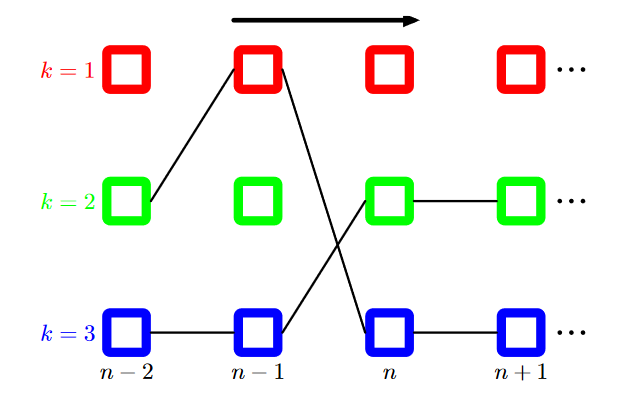
\includegraphics[scale=0.3]{images/09_BayesianNetworksInference_trellis.png}
	\caption{Trellis for linear chain}
	\label{fig:trellis}
\end{figure}
A trellis diagram shows $k$ possible states of a variable (in this case $k=3$), the
states for each node are represented in $n$ columns, times goes left to right. For
each state $k$ of a variable $X_{n}$, $\Phi_{f_{n-1, n} \rightarrow X_n}(X_{n})$
defines a unique state which is maximal given the previous states (in the diagram
is linked by an edge). Once the maximal states for the last variable $X_{n}$ is chosen,
that I back-propagate through the links in order to get the most probable
configuration of the previous nodes. \\ This procedure works also for trees with
the exception that we need to back-propagate multiple times. The reasoning is
still the same.

\sumup{This is needed because if I want the most probable explanation, I do not just want the probability but I am also interested in the most probable configuration for that to happen. Therefore I propagate the probability message $\mu$ and the configuration message $\Phi$.}

\subsubsection{Underflow issue}
When we compute products of probabilities ($0 < p < 1$) the number becomes
smaller and smaller: therefore we can get across the \textit{underflow issue}. In
order to avoid this problem we typically use the $\log$ since it is monotonic and
allows to replays multiplication with summation.

\subsection{Exact inference on general graphs}
These algorithm can not be applied on graphs that do not produce tree-structure factor
graphs. If we have BN that do not satisfy these conditions (like containing undirected
loops) these algorithms can not be applied anymore but there are very similar
algorithms (that use slightly similar intermediate structures as \textit{junction
trees} instead of factor graphs). In junction trees the nodes contain clusters
of variables (which can contain loops) and the apply the very same idea
described in the previous paragraphs. This algorithm becomes exponential with the
size of the cluster. What happens in reality is that we need to approximate
because we can not afford exact inference in these cases. There is a lot of research
going on that looks for the best way to approximate inference such as:
\begin{itemize}
	\item \textbf{looply belief propagation} that consists in message passing on
		the original graph even if it contains loops

	\item \textbf{variational methods} that are deterministic approximations
		assuming the posterior probability factorizes in a particular way

	\item \textbf{sampling methods} that approximate posterior with getting
		samples from the network
\end{itemize}
In the looply belief propagation we build a factor graph, the message flows indefinitely.
This methods allows the message passing through loops deciding a scheme of
message sending. The node possibly recomputes some messages, this implies that
for every iteration, values are recomputed. If the value shrinks, the network is
converging (all messages do not change), but there is no guarantee that this
will happen. The maximal configurations and maximum probabilities will not be exact
but approximations. \\

In the sampling methods, I get a set of configuration of this network which is
compatible with the probability. Then we can sample from the distribution and check
if they are compatible with the configuration we intend to verify. It is tricky
to sample from the distribution. So what we do is Monte Carlo Markov Chain (MCMC):
we do not sample from posterior, but from a random process that get progressively
closer to the posterior. This means that the state of the process is a
configuration, and a new state is generated from moving some variables (change
of state). We move in this space according to a probabilistic model, given certain
conditions, it converges to a configuration that can be used as samples.